\documentclass[ignorenonframetext,]{beamer}
\usepackage{amssymb,amsmath}
\usepackage{ifxetex,ifluatex}
\ifxetex
  \usepackage{fontspec,xltxtra,xunicode}
  \defaultfontfeatures{Mapping=tex-text,Scale=MatchLowercase}
\else
  \ifluatex
    \usepackage{fontspec}
    \defaultfontfeatures{Mapping=tex-text,Scale=MatchLowercase}
  \else
    \usepackage[utf8]{inputenc}
  \fi
\fi
% Redefine labelwidth for lists; otherwise, the enumerate package will cause
% markers to extend beyond the left margin.
\makeatletter\AtBeginDocument{%
  \renewcommand{\@listi}
    {\setlength{\labelwidth}{4em}}
}\makeatother
\usepackage{enumerate}
% Comment these out if you don't want a slide with just the
% part/section/subsection/subsubsection title:
\AtBeginPart{\frame{\partpage}}
\AtBeginSection{\frame{\sectionpage}}
\AtBeginSubsection{\frame{\subsectionpage}}
\AtBeginSubsubsection{\frame{\subsubsectionpage}}
\setlength{\parindent}{0pt}
\setlength{\parskip}{6pt plus 2pt minus 1pt}
\setlength{\emergencystretch}{3em}  % prevent overfull lines
\setcounter{secnumdepth}{0}
% header.tex - DESC
% Iago Mosqueira - JRC. 2012
%

%
%\def\input@path{{/path/to/folder}}

% packages
\usepackage[absolute,overlay]{textpos}

\setlength{\TPHorizModule}{\paperwidth}
\setlength{\TPVertModule}{\paperheight}

%% gets rid of navigation symbols
\setbeamertemplate{navigation symbols}{}

%% bullet points
\setbeamertemplate{itemize items}[circle] % if you want a ball
\setbeamertemplate{itemize subitem}[circle] % if you wnat a circle
\setbeamertemplate{itemize subsubitem}[circle] % if you want a triangle

%% colors {{{
\definecolor{ecblue}{RGB}{1,70,147}
\definecolor{jrcblue}{RGB}{55,172,222}
\setbeamercolor{normal text}{fg=black,bg=white}
\setbeamercolor{structure}{fg=ecblue} 
\setbeamercolor{shadedhead}{bg=jrcblue}
\setbeamercolor{shadedcover}{bg=ecblue,fg=yellow}
% }}}

%% images {{{
% footer
\pgfdeclareimage[height=5.5mm]{footer}{tex/footer}

% header
\pgfdeclareimage[width=0.1575\paperwidth]{header}{tex/header}

% headerT
\pgfdeclareimage[width=0.1575\paperwidth]{headerT}{tex/headerT}

% title page image
\pgfdeclareimage[width=0.6\textwidth]{titlegraphic}{graphics/front}
% }}}

%% title page {{{
\setbeamertemplate{title page}{

% title block
\begin{textblock}{0.7}[0,0](0.15,0.2)
\centering
{\fontsize{18}{26}\selectfont
\bfseries
\color{ecblue}\inserttitle}
\end{textblock}

% author block
\begin{textblock}{0.5}[0,0](0.55,0.55)
{\fontsize{12}{16}\selectfont
\color{black}
FISHREG\\
Maritime Affairs Unit - IPSC\\
European Commission\\
Joint Research Center\\
}
\vfill
\end{textblock}

% picture block
\begin{textblock}{0.5}[0,0](0,0.47)
 \pgfuseimage{titlegraphic}
\end{textblock}

} % }}}

%% headline {{{
\setbeamertemplate{headline}{
\leavevmode\hbox{%
%% uniform box
\begin{beamercolorbox}[wd=\textwidth,ht=0.1447\paperheight,dp=0ex]{shadedhead}%
	%% EC logo
	\centering
	%% 0.02895
  \vspace{-0.044\paperheight}
	\pgfuseimage{header}
\end{beamercolorbox}%
}} % }}}

%% frame title {{{
\setbeamertemplate{frametitle}
{
\color{jrcblue}\vspace{2ex}\fontsize{12}{16}\selectfont
\textbf{\insertframetitle}
\par
} % }}}

%% footline {{{
%% left: date as in title
\newcommand{\footlinetext}{\insertdate}
\setbeamertemplate{footline}{
\begin{minipage}{58mm}
\hspace{7.5mm} \footlinetext
\end{minipage}
\hspace{0.1mm}
%% center: jrc logo
\begin{minipage}{8.5mm}
 \pgfuseimage{footer}
\end{minipage}
\hspace{0.1mm}
%% right: page number
\begin{minipage}{50mm}
 \flushright \insertframenumber
\end{minipage}
} % }}}

\title{Training Course \textbf{USING FLR FOR QUANTITATIVE FISHERIES ADVICE}}
\author{FISHREG - European Commission Joint Research Centre}
\date{March 2013}

\begin{document}
\frame{\titlepage}

\begin{frame}\frametitle{Welcome to (almost) the EC JRC, Ispra, Italy.}

\centering
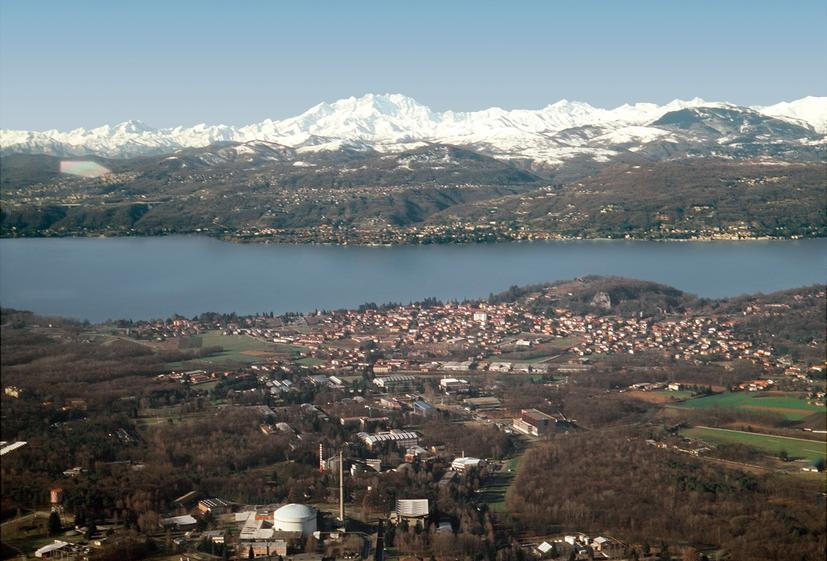
\includegraphics[keepaspectratio, width=0.8\textwidth]{graphics/jrcispra.png}

\end{frame}

\begin{frame}\frametitle{AGENDA}

\begin{itemize}
\item
  TIMETABLE: 9.00 - 12.30 / 14.00 - 17.30
\item
  BREAKS @ 10.30 / 15.30
\end{itemize}
\end{frame}

\begin{frame}\frametitle{LOGISTICS}

\begin{block}{Lunch}

\begin{itemize}
\item
  Don Guanella
\end{itemize}
\end{block}

\begin{block}{Dinner}

\begin{itemize}
\item
  Don Guanella
\item
  Other places
\item
  Course dinner THU
\end{itemize}
\end{block}

\end{frame}

\begin{frame}\frametitle{MATERIALS}

\begin{itemize}
\item
  R 2.15.*
\item
  RStudio or other text editor
\end{itemize}
\end{frame}

\begin{frame}\frametitle{INSTALLATION}

\begin{block}{Select 32 bit R}

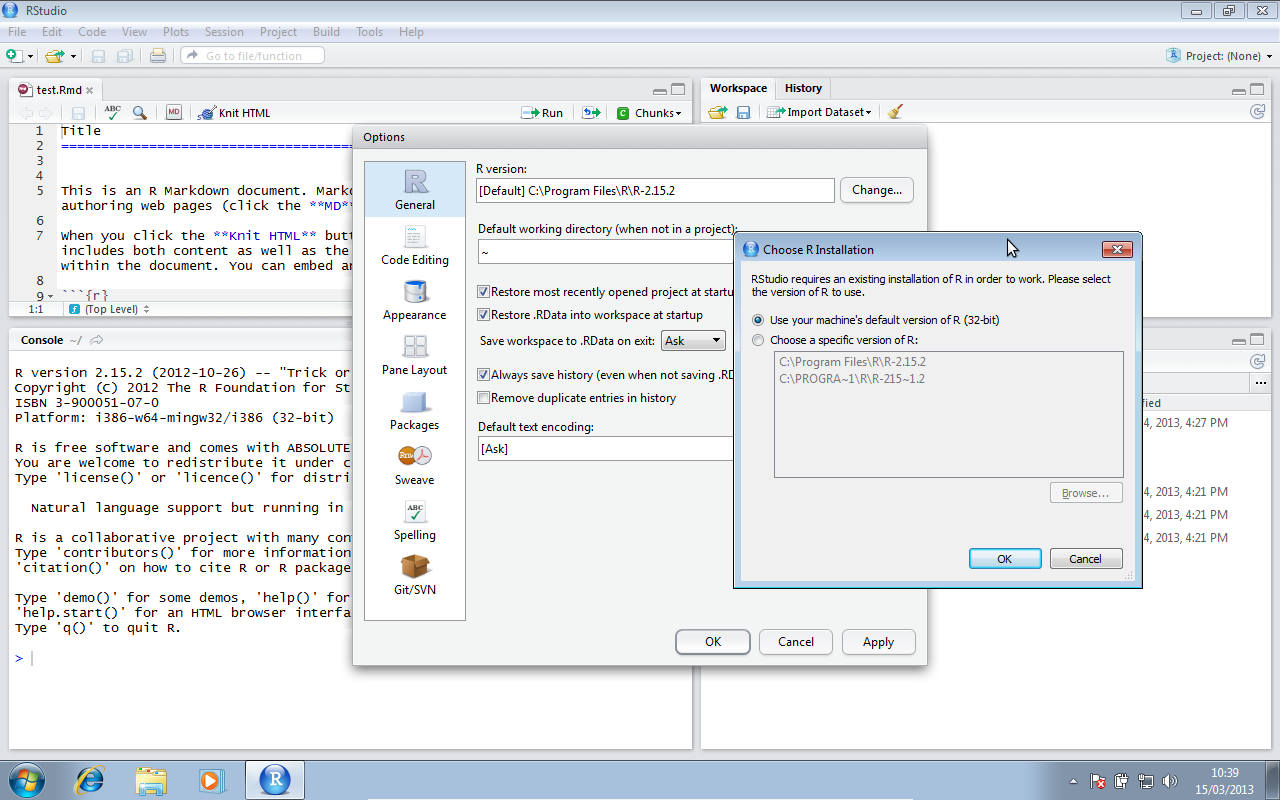
\includegraphics[keepaspectratio, width=\textwidth]{graphics/RStudio.png}

\end{block}

\end{frame}

\begin{frame}[fragile]\frametitle{INSTALLATION: packages}

\texttt{install.packages("")}

\begin{itemize}
\item
  \texttt{akima}
\item
  \texttt{ggplot2}
\item
  \texttt{plyr}
\item
  \texttt{knitr}
\item
  \texttt{RcppArmadillo}
\end{itemize}
\end{frame}

\begin{frame}[fragile]\frametitle{INSTALLATION: packages}

\texttt{install.packages(repos="http://flr-project.org/Rdevel")}

\begin{itemize}
\item
  \texttt{FLCore}
\item
  \texttt{FLEDA}
\item
  \texttt{FLash}
\item
  \texttt{ggplotFL}
\item
  \texttt{FLBRP}
\item
  \texttt{FLAssess}
\item
  \texttt{FLa4a}
\item
  \texttt{FLXSA}
\item
  \texttt{SQLiteFL}
\end{itemize}
\end{frame}

\begin{frame}\frametitle{OUTLINE}

\begin{enumerate}[1.]
\item
  Introduction to FLR
\item
  Load data and EDA
\item
  Introduction to modelling: FLSR
\item
  Stock assessment
\item
  Reference points
\item
  Forecasting
\item
  Simulation
\item
  A Case study
\end{enumerate}
\end{frame}

\begin{frame}\frametitle{HOW WILL IT RUN}

\begin{itemize}
\item
  Presentations
\item
  Tutorials
\item
  Exercises
\item
  Paper of the day
\end{itemize}
\end{frame}

\begin{frame}\frametitle{Today's paper}

Kell, L. T., Mosqueira, I., Grosjean, P., Fromentin, J-M., Garcia, D.,
Hillary, R., Jardim, E., Mardle, S., Pastoors, M. A., Poos, J. J.,
Scott, F., and Scott, R. D. 2007. FLR: an open-source framework for the
evaluation and development of management strategies. -- \emph{ICES
Journal of Marine Science}, 64: 640--646.

\centering

\includegraphics[keepaspectratio, height=0.6\textheight]{graphics/kelletal.png}

\end{frame}

\begin{frame}\frametitle{LICENSE}

\begin{block}{Presentations: Creative Commons Attribution-ShareAlike 3.0
License.}

\centering

\includegraphics[keepaspectratio, width=0.3\textwidth]{graphics/cc-by-sa.png}

\end{block}

\begin{block}{Code: General Public License 3.0}

\centering

\includegraphics[keepaspectratio, width=0.3\textwidth]{graphics/gpl3.png}

\end{block}

\end{frame}

\begin{frame}\frametitle{ABOUT US}

\begin{block}{Ernesto Jardim - STECF, MPs, a4a}

\end{block}

\begin{block}{Colin Millar - a4a, MPs}

\end{block}

\begin{block}{Iago Mosqueira - FLR, IOTC, MPs}

\end{block}

\begin{block}{Chato Osio - MED, STECF}

\end{block}

\begin{block}{Finlay Scott - BioEco, FLR}

\end{block}

\end{frame}

\begin{frame}\frametitle{READY !!}

`Men learn while they teach.'

Seneca the Younger

\end{frame}

\end{document}
